\documentclass[11pt]{informatics-report}
\usepackage{color}
\usepackage[square,sort,comma,numbers]{natbib} 
\usepackage{comment}
\usepackage{url}
\usepackage{graphicx}
\usepackage{cleveref}
\usepackage{hyperref}
\graphicspath{ {Diagrams/}}


\title{6CCS3PRJ Final Year\\\vspace{0.2cm} LOST}
\author{Joshua Simpson}
\studentID{1225043}
\supervisor{Andrew Coles}

\date{\today}

\abstractFile{FrontMatter/abstract.tex}
\ackFile{FrontMatter/acknowledgements.tex} 

\begin{document}
\createFrontMatter
\onehalfspacing
\tableofcontents
\doublespacing


\chapter{Introduction}
Location based services have been developing over the past few decades, and are prevalent in several aspects of every day life - location based services range from the route-planning software that is used to figure out a morning commute, to live time-tabling services that use bus or train positions to give accurate estimates. It is safe to say that in some way or another, location services are prevalent in modern day life.

However, GPS\footnote{ Global Positioning System - a system using satellites to provide precise location information} services only work to a certain level;  specifically, they only work to within a few feet at street level\cite{cook2005indoor}. Whilst this is still a feat, it leaves a large market gap for contextually aware services inside large buildings. 

Contextually aware services are another rapidly developing technology, providing users with information or activities specific to their current location or situation, determining the suitability for such events by using sensor data\footnote{ Data such as location, temperature or time }. 

There are previous studies on using local area wireless access points to provide this sensor data at a level more precise than GPS can currently allow, but they are usually run in controlled environments, deriving a single mathematical equation in order to determine distance from the access point with high precision\cite{996891}. Unfortunately, this is impractical to apply as general use outside of a test environment.
\newline \newline 


\section{Project Aims}

The main goal of this project is to provide a proof-of-concept mobile application that can provide location and route-planning services whilst also delivering contextually aware services in a specific building - all without using GPS - demonstrating the possibilities that this area of application development holds for developers. Around this main feature, the project will aim to create software suite allowing for the efficent setup of a 'contextually aware building', as well as provide practical functionality to a variety of user groups ( by using the application to crowdsource data), to demonstrate the potential in this field. To achieve this, I will be collecting data on user location and wifi failure\footnote{A common occurence in the chosen building} throughout the building and providing a backend that displays this data in a useful manner.

To demonstrate a successful project, a large building with many potential locations is useful, as it shows the accuracy of of the location-finding and route-planning algorithms. To this end, the building that I am using to test this application is King's College London's Strand Campus\footnote{ It has not escaped my attention that this will also help all the new first years find Waterfront}. With roughly 17,000m2 of space and 9 floors to utilise, the application would not only be thoroughly tested but also most likely welcomed by King's 25,000 students\cite{headcount}.

\section{Report Structure}

This report will begin with a background on the project - taking a look at location based services and contextually aware services and the applications of both that are already available, along with an analysis of projects or papers that have attempted to solve the problem of location services at building level. This data will then be collated to analyse key problem areas during implementation. 

Following this there will be an outline of the requirements and specification for the project - showing both the project itself and the chosen extensions - complete with justifications on decisions made in the specification.


\chapter{Project Background and Main Points to Consider}

\section{Location Services}

Defined as \textit{"services that integrate a mobile device's location or position with other information so as to provide added value to a user"}\cite{schiller2004location}, the origins of location information services date back to 1973, when the US Department of Defence developed GPS to overcome the limitations imposed by navigation systems in use at the time\cite{national1995global}. This original system has since been developed into an integral part of many mobile applications, including mapping and route planning applications, as well as forming the 'sensor' in a lot of contextually aware applications. There is a well established method that is used in order to ascertain location, called trilateration\footnote{The process of finding a location by measuring distances, using geometry}. Triangulation\footnote{The process of finding a location by estimating the direction in which signals are coming from} is another method used to determine location, but is mostly inapplicable in the context of mobile devices\footnote{It is also commonly mistaken for trilateration}. Whilst I will not be developing an application that directly uses existing location technologies such as GPS, it is important to consider the practices used in such technologies when developing this project.

\subsection{Application: Google Maps}

Google Maps is easily the most widely used mapping tool on the planet, with over 54\% of smartphone owners using the app on a regular basis in 2013 ( for comparison, this was 10\% more than Facebook at the time)\cite{googlemaps}. Google Maps are a chief provider of location information services, with advanced route planning and street-view functionality. They serve this data through their own API\footnote{https://developers.google.com/maps/}. The most interesting aspect of their service ( in relation to this paper, at least ) is their recent addition of the use of Wireless Access Points for their location services. Whilst they do not rely solely on it for location, they do use the data to increase accuracy and speed through their Maps application\cite{googlewifi}. Interestingly, Google collect this WiFi data by crowdsourcing through an 'opt out' scheme in the Google Maps application\cite{googlewifi2} - this may not be possible in the case of this project ( as Google have used WiFi in a more assistive manner ), but it provides a good basis from which to approach the problem.

\subsection{Paper: Indoor Location Using Trilateration Characteristics}\cite{cook2005indoor}

This paper is especially relevant to the problem, considering the use of Wireless Local Area Networks in order to achieve trilateration. This is achieved by measuring the signal strength for at least 3 access points, and using the signal strength to determine the distance from the access point. Once you have three accurate distances you can essentially create a 'Venn Diagram' of where the user is located.

The paper goes on to state that there are inherent inaccuracies with this positioning technique, due to the variable nature of radio signals\cite{cook2005indoor}. 

To circumvent these inaccuracies, an elegant averaging method was developed, which started returning an accurate 'average signal strength' after 40 readings.

\subsubsection{Issues with the trilateration approach}
- As stated above, the trilateration approach has difficulties providing accuracies:

\textit{"Radio signals are extremely variable, particularly indoors, due to being reflected by obstacles or refracted round corners, known as multipath reflection. Environmental changes can also affect the signals, such as the number of people around. This means that the positioning technique is inherently inaccurate, with positions from raw Wi-Fi signals being in excess of 10m out. "}\cite{cook2005indoor}

\noindent- Whilst there is a solution designed to solve this problem in the case of the test environment, an application in a building such as Kings would require a number of different formulae in order to provide accurate signal strength averaging for different areas of King's\footnote{ Because of the variables such as distance between routers, building material, and the number of users in any area at a given time}

\noindent- Finally, in cases where the averaging solution is easily applicable, there \textit{should} be concerns regarding the impact on a mobile device's battery life when performing repeated scans and operations on the results of those scans.

\subsection{Paper: More Stuff on Location - Fuzzy Location?} 

\section{Context-Aware Services}

Contextually aware services are services that use data that pertains to the user or application's current situation to provide actions or functionality specific to that scenario. It is defined by Abowd as 

\textit{ "any information that can be used to characterize the situation of entities (i.e., whether a person, place or object) that are considered relevant to the interaction between a user and an application, including the user and the application themselves." }\cite{abowd1999towards}

Contextually aware services use 'sensors' to fetch this information - examples include location data, temperature, even the camera on your phone could be used as a sensor for contextual services\footnote{Consider how recent smartphones have software that stops the screen coming out of standby if it thinks it is in your pocket}.

\subsection{Estimote}

A rapidly accelerating tech start up, Estimote provides 'beacons' using low-power Bluetooth in order to send an ID\footnote{\url{http://estimote.com/api/getting-started/intro-to-beacons.html}} to an Estimote enabled application - these can then be programmatically associated with locations, events, etc. and calculates its distance from the phone using RSSI ( the received signal strength ) inside it's own API, meaning that it can be used very effectively to provide location-based services with minimal effort. This is so far the the most prominent product in the market using the iBeacon base.

Currently the major drawback of the Estimote is the price, which limits Estimote beacons / stickers to small buildings – covering an area such as King’s would be incredibly costly\footnote{\url{http://estimote.com/\#jump-to-products}}, and any structural changes regarding the beacons would require significant effort to represent in an application developed to use Estimote. Another issue is that - as stated above - using RSSI to fetch location information can become very complex in a large building with lots of people in it (which would cause signal attenuation at different levels throughout the day). 

\subsection{Google Maps}

As part of their vast toolset, Google Maps also has context-sensitive functions in it's API - an example is their 'Explore' feature\footnote{\url{http://google-latlong.blogspot.co.uk/2014/07/spend-more-time-exploring-with-google.html}}, which will show destinations of a certain type that are in the user's local area. The Explore function even takes into account time of day and weather in order to provide the best possible locations to the user.

An interesting point to note is that the 'Explore' function was predated by a 'Search Nearby' function that was removed\footnote{\url{http://www.jsonline.com/blogs/news/247119811.html}} - possibly due to privacy concerns\footnote{Covered later in Ethical Concerns}.


\subsection{Paper: An Architecture for Data Collection and Processing in Context-Aware Applications}\cite{salviarchitecture}

In this paper, Dario Salvi \textit{et al} pose that whilst Context Aware systems are showing and developing a greater use in general applications, that the field is not "applied in the real world"\cite{salviarchitecture}. The paper then goes on to propse an architecture that access and uses contextual data differently to provide the developer with more possibility to develop what is referred to as 'real world applications'.

Afterwards, the writers go on to set out three classes for collecting data - AtomicData\footnote{Singular pieces of information}, ContextData\footnote{Compositions of more than one piece of AtomicData}, and Relationships\footnote{Links between two ContextData}\cite{salviarchitecture}. These classes provide an interesting base for the data collection part of this project\footnote{ContextData holds the most interest, as I will need to collect multiple pieces of data}.

Overall the paper presents some very useful points on using contextual data to return usable information.

\section{Crowd Sourcing}

Crowd sourcing is generally defined as using a group of people or community to generate a needed resource. It is mostly thought of in terms of popular crowd-funding sites such as Kickstarter, or Indiegogo, but the term extends to other resources, such as data or ideas\footnote{For example, Cracked.com - a satire website - uses its own staff, but also looks for stories contributed by it's readers}. Generally, data crowdsourcing follows a pattern of clients paying for information that they need, and users that receive rewards to collect or generate this information.

\subsection{Captcha} 

Captcha was originally invented as an identification system to help discern humans from robots when performing tasks online. This started out as just a verification system ( which is growing more and more elaborate as robots evolve ), but was eventually evolved into an aid to digitizing books\footnote{\url{http://www.npr.org/2013/10/04/191620023/can-you-crowdsource-without-even-knowing-it}}. The most interesting point about this is that most of the users of Captcha have no idea that they are crowd-sourcing a huge effort every time they solve a Captcha.

\subsection{The 90-9-1 Rule for Participation Inequality in Social Media and Online Communities}\cite{participationinequality}

This article addresses a major problem with crowdsourcing data which Nielsen refers to as participation inequality, stating that user participation often follows a 90-9-1 rule, with 90\% of users being "lurkers or users that will observe but not contribute"\cite{participationinequality} . Nielsen also covers how to overcome this participation inequality (after briefly summarizing with ‘you can’t’); one method in particular is of interest when considering the aims of this project and its associated application: 'make participation a side effect'  – essentially the act of collecting data without the user having to do anything - this is less intrusive to the user’s day-to-day use of the application, but can also have obvious ethical ramifications if the user is unaware if they are sourcing data.

\section{Platform}

Because of the nature of the application being developed, it makes the most sense to develop for a mobile device - whilst devices like laptops offer more power to process information, the dataset that needs to be taken does not require the extra resources. Alongside this, mobile devices lend themselves better to the data-collection aspect of the project, with background services that can perform operations whilst the phone is inactive in a user's pocket. Finally, it is easier for a user to take out their phone in order to ascertain their location than it would be for a user to take out their laptop to perform the same operation.

With this in mind, the choice of platform then comes down to which type of mobile device to develop for - Android devices, or iOS devices. Whilst I could develop for both device types simultaneously using a platform such as Phonegap\footnote{http://phonegap.com/}, I have concerns about not using the native SDK for a platform - the abstraction provided by platforms such as Phonegap may reduce or restrict functionality that is necessary during development\footnote{Phonegap as an example, uses HTML, CSS and Javascript to create an application for both platforms simultaneously}. In the end, I decided to develop this for the Android platform alone.

\subsection{Reasons for Android as a platform}

The first point I considered whilst choosing a platform to use is the popularity of a platform - it makes sense to make the application available to the widest audience possible. In this case, Android dominates the market share, with 76.6\% of smartphones using the Android OS, compared to 19.7\% using iOS in the last quarter of 2014\cite{devicestats}.

Another major concern when deciding upon device was the functionality provided by SDKs for both Android and iOS. When I reviewed the functionality for both devices, I was unsurprised to find that iOS does not allow access to lower-level functionality. What did surprise me is that statistics like wireless signal strength was amongst these lower level functions\cite{ios1}\cite{ios2}\footnote{Whilst StackOverflow is not preferable as a citable source, finding an admission from Apple on this point is very difficult}. This restriction of access was a major concern\footnote{Unfortunately, later modifications to the application to circumvent issues with using signal strength meant this was no longer an issue}

\section{Ethical Concerns}

When developing an application that uses any form of personal information, there are definite privacy concerns. This is exascerbated when considering that there will be location information being returned to a server that is accessible by staff members. In this respect, it is important to not only adhere strictly to Data Protection laws, but also to consider the user's privacy and wellbeing. To this end, I need to make sure to collect the least amount of data I can, and to anonymise this data as much as possible in order to avoid sending any user details that would affect their privacy. Alongside this it would be prudent to secure the repository of any stored data against unauthorised users.

Another ethical point to consider is the code that is used to create this application. I should take due care to create this app using only my own code, except where express permission has been granted. In the same vein, I must make sure to adhere to all licenses for any libraries which I use in development.

\chapter{Requirements}
The client end of this project consists of two parts - an Android application that can determine user location ( LOST ) and provide route-planning inside the building, whilst feeding data to the backend, which will store the data and provide functions to view it as information. Alongside this, I will develop a secondary Android application ( FOUND ) so that I can easily collect wireless data to test the application with. FOUND will not be available for users of the resulting software package for this project, however when considering possible extensions after the BSc report, FOUND would be an active component to allow for the easy mapping of a building in a bespoke software package.

\section{LOST - Android Application}

\subsection{Functional Requirements}
\begin{description}
\item[F1] - The application will be able to retrieve the most recent SQLite database containing wireless access point location information upon startup.
\item[F2] - The application will be able to accurately discern the user's location, using data provided by an SQLite database.
\item[F3] - The application will be able to provide the user with route-planning data, allowing the user to select a start and an end point, and provide the shortest path between the two points.
\item[F4] - The application will be able to discern whether the device is currently in the correct building for usage.
\item[F5] - The application will send anonymous information on the user's location to the backend periodically, if it is in the correct building
	\begin{description}
	\item[F5.1] - The user will be able to turn off this functionality
	\end{description}
\item[F6] - The application will periodically check if it has a functioning internet connection - if it is in the correct building. If the internet connection is malfunctioning, it will save this data.
	\begin{description}
	\item[F6.1] - Once the application regains internet access, it will send location data, and the MAC address of malfunctioning router to the backend.
	\item[F6.2] - The user will be able to turn off this functionality.
	\end{description}
\end{description}
\subsection{Non-functional Requirements}
\begin{description}
\item[NF1] - Application will not cause an 'ANR' ( app not responding ) error on any 'low-end' smartphone ( at time of writing, low end specifications are considered to be 1Ghz dual core processor and 768mb RAM\footnote{Figures created by comparing phone specifications at \url{http://www.phonearena.com/news/Affordable-not-cheap-15-best-low-cost-smartphones_id58696}}).
\item[NF2] - Application will provide location accurate to within 20 feet.
\item[NF3] - Application will use as little battery life as possible, using less than 5\% battery life within an hour.
\item[NF4] - Application will minimise data usage, making sure not to post data back using mobile data.
\item[NF5] - Application will not send data that can be used to identify the user, or any information that may be personal to the user / a breach of Data Protection laws.
\end{description}

\section{Backend}
\subsection{Functional Requirements}
\begin{description}
\item[F1] - Backend will operate a RESTful API that will allow the mobile application to post data to the server
\item[F2] - Backend will store POSTed data to an SQL database
\item[F3] - Backend will be retrieve data from SQL database, and display to user as information
\item[F4] - Backend will require user authentication to allow access to displayed data
\item[F5] - Backend will be able to store wifi location database, and serve it to a mobile device
\end{description}

\subsection{Non-functional Requirements}

\begin{description}
\item[NF1] - Backend will provide an easily navigable user interface
\item[NF2] - Backend will show data in an easily readable manner
\end{description}

\section{FOUND - Android Application}

\subsection{Functional Requirements}

\begin{description}
\item[F1] - Application will scan local wifi access points
\item[F2] - Application will insert the top access point into an SQLite database as a node, along with an edge connecting it to another node in the directed graph
\end{description}

\chapter{Design}
The application is split into two parts - therefore it will be detailed as a whole product, before the design of each component is analysed individually. Generally, the backend and the frontend application work as their own components, with the only interaction between the two being fetching the database, and sending data from the application to the database; because of this, an agile development cycle will be used. 

Further to this, a basic version of the Android application will be developed first, and an inital deployment of the backend, with the ability to receive data from the mobile application after that - from then, incremental additions will be made to either component, building for functionality first, then returning later for optimisation. 
\newpage

\section{Component Diagram}
\centerline{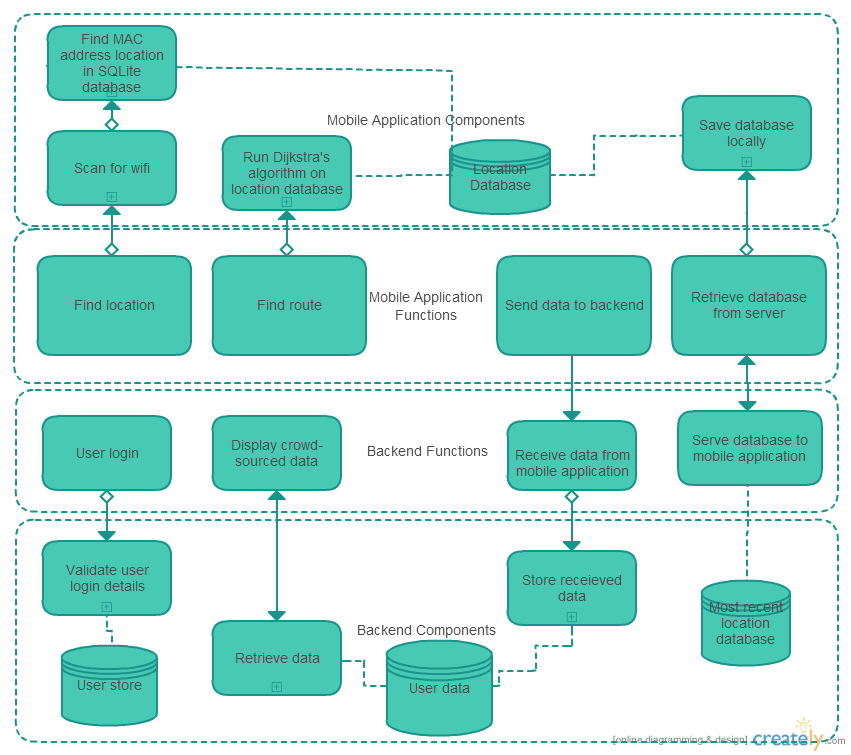
\includegraphics[scale=0.6]{ComponentDiagram}}
\newpage

\section{LOST}

The 'front end' of the project, the LOST application provides most of the functionality detailed in the earlier chapters of this report. In this section, I will go into more detail as to what each function will need to do in order to provide the outlined functionality. You will find a \nameref{UseCase}, along with wireframes for each aspect in the Appendix. For clarification, each 'view' in an Android Application is called an Activity.

\subsection{Finding Location}

This is one of the most critical aspects of the application, and also one of the most challenging as a great deal of consideration needs to be paid towards efficiency, accuracy, and precision - it will generally be more expensive in terms of resources, and in fact battery power, to increase the precision.

In order to ascertain location, the application will need to perform a scan of nearby wireless access points. The MAC address and signal strength of each access point will be collected, and put in descending\footnote{Or considering how signal strengths are measure, ascending. Signal strength is measured in DBm and measure as negative figures. The 'quieter' a signal is, the weaker it is - therefore a signal strength of -10 is much more powerful than a signal strength of -80} order of strength.
The original intention\footnote{Results of this will be detailed in the 'Implementation' section of this report.} at this point was to use actual signal strength figures to get the most precise location information, as done by Cook \textit{et al}\cite{cook2005indoor}. 

To get this location information, the top three MAC addresses in the list would be used to filter the location database down to a single node, representing that location\footnote{Discussed further in the Databases section}. This location would then be displayed to the user, along with an option to refresh this ( performing another scan, incase the user doesn't think they are in the right location ). There will also be a button that allows the user to use their given location as the start or end point for route planning.

\subsection{Route Planning}

This function ties in with the location finding function of the application - the user will either be able to load it normally, or load it from the 'Location Finder' part of the application - if this is the case then either the 'to' or 'from' sections of the application will contain the user's location.

Regardless of how the activity is accessed, there will be two drop down lists, allowing the user to select the start and end points. The application will translate these selections into nodes in the directed graph created from the location database, and perform Dijkstra's algorithm to find the shortest path between the two locations. The nodes traversed in this path are displayed on the next Activity to show the user the path they need to take.

\subsection{Data Upload}

This function will run at regular intervals in the background, regardless of whether the app is open, as the chances of the user having the app open all the time are very slim - an average app sessions lasts barely more than a minute\cite{Bohmer:2011:FAA:2037373.2037383}. 

%\chapter{Report Body}
The central part of the report usually consists of three or four chapters detailing the technical work undertaken during the project. {\bf{\textcolor{red}{The structure of these chapters is highly project dependent}}}. They can reflect the chronological development of the project, e.g. design, implementation, experimentation, optimisation, evaluation, etc (although this is not always the best approach). However you choose to structure this part of the report, you should make it clear how you arrived at your chosen approach in preference to other alternatives. In terms of the software that you produce, you should describe and justify the design of your programs at some high level, e.g. using OMT, Z, VDL, etc., and you should document any interesting problems with, or features of, your implementation. Integration and testing are also important to discuss in some cases. You may include fragments of your source code in the main body of the report to illustrate points; the full source code is included in an appendix to your written report.

\section{Section Heading}

\subsection{Subsection Heading}
%\chapter{Design \& Specification}

\section{Section Heading}
%\chapter{Implementation}

\section{Section Heading}

%\chapter{Professional and Ethical Issues}
Either in a seperate section or throughout the report demonstrate that you are aware of the \textbf{Code of Conduct \& Code of Good Practice} issued by the British Computer Society and have applied their principles, where appropriate, as you carried out your project.

\section{Section Heading}

%\chapter{Results/Evaluation}

\section{Software Testing}

\section{Section Heading}

%\chapter{Conclusion and Future Work}

The project's conclusions should list the key things that have been learnt as a consequence of engaging in your project work. For example, ``The use of overloading in C++ provides a very elegant mechanism for transparent parallelisation of sequential programs'', or ``The overheads of linear-time n-body algorithms makes them computationally less efficient than $O(n \log n)$ algorithms for systems with less than 100000 particles''. Avoid tedious personal reflections like ``I learned a lot about C++ programming...'', or ``Simulating colliding galaxies can be real fun...''. It is common to finish the report by listing ways in which the project can be taken further. This might, for example, be a plan for turning a piece of software or hardware into a marketable product, or a set of ideas for possibly turning your project into an MPhil or PhD.


\bibliographystyle{plain}
\bibliography{mybib}
\addcontentsline{toc}{section}{Bibliography}


\appendix
\include{Appendices/appendix}
%\chapter{User Guide}
\section{Instructions}
You must provide an adequate user guide for your software. The guide should provide easily understood instructions on how to use your software. A particularly useful approach is to treat the user guide as a walk-through of a typical session, or set of sessions, which collectively display all of the features of your package. Technical details of how the package works are rarely required. Keep the guide concise and simple. The extensive use of diagrams, illustrating the package in action, can often be particularly helpful. The user guide is sometimes included as a chapter in the main body of the report, but is often better included in an appendix to the main report.

%\chapter{Source Code}
\section{Instructions}
Complete source code listings must be submitted as an appendix to the report. The project source codes are usually spread out over several files/units. You should try to help the reader to navigate through your source code by providing a ``table of contents'' (titles of these files/units and one line descriptions). The first page of the program listings folder must contain the following statement certifying the work as your own: ``I verify that I am the sole author of the programs contained in this folder, except where explicitly stated to the contrary''. Your (typed) signature and the date should follow this statement.

All work on programs must stop once the code is submitted. You are required to keep safely several copies of this version of the program - one copy must be kept on the departmental disk space - and you must use one of these copies in the project examination. Your examiners may ask to see the last-modified dates of your program files, and may ask you to demonstrate that the program files you use in the project examination are identical to the program files you had stored on the departmental disk space before you submitted the project. Any attempt to demonstrate code that is not included in your submitted source listings is an attempt to cheat; any such attempt will be reported to the KCL Misconduct Committee.

\textbf{You may find it easier to firstly generate a PDF of your source code using a text editor and then merge it to the end of your report. There are many free tools available that allow you to merge PDF files.}


\end{document}
